\documentclass[1p]{elsarticle_modified}
%\bibliographystyle{elsarticle-num}

%\usepackage[colorlinks]{hyperref}
%\usepackage{abbrmath_seonhwa} %\Abb, \Ascr, \Acal ,\Abf, \Afrak
\usepackage{amsfonts}
\usepackage{amssymb}
\usepackage{amsmath}
\usepackage{amsthm}
\usepackage{scalefnt}
\usepackage{amsbsy}
\usepackage{kotex}
\usepackage{caption}
\usepackage{subfig}
\usepackage{color}
\usepackage{graphicx}
\usepackage{xcolor} %% white, black, red, green, blue, cyan, magenta, yellow
\usepackage{float}
\usepackage{setspace}
\usepackage{hyperref}

\usepackage{tikz}
\usetikzlibrary{arrows}

\usepackage{multirow}
\usepackage{array} % fixed length table
\usepackage{hhline}

%%%%%%%%%%%%%%%%%%%%%
\makeatletter
\renewcommand*\env@matrix[1][\arraystretch]{%
	\edef\arraystretch{#1}%
	\hskip -\arraycolsep
	\let\@ifnextchar\new@ifnextchar
	\array{*\c@MaxMatrixCols c}}
\makeatother %https://tex.stackexchange.com/questions/14071/how-can-i-increase-the-line-spacing-in-a-matrix
%%%%%%%%%%%%%%%

\usepackage[normalem]{ulem}

\newcommand{\msout}[1]{\ifmmode\text{\sout{\ensuremath{#1}}}\else\sout{#1}\fi}
%SOURCE: \msout is \stkout macro in https://tex.stackexchange.com/questions/20609/strikeout-in-math-mode

\newcommand{\cancel}[1]{
	\ifmmode
	{\color{red}\msout{#1}}
	\else
	{\color{red}\sout{#1}}
	\fi
}

\newcommand{\add}[1]{
	{\color{blue}\uwave{#1}}
}

\newcommand{\replace}[2]{
	\ifmmode
	{\color{red}\msout{#1}}{\color{blue}\uwave{#2}}
	\else
	{\color{red}\sout{#1}}{\color{blue}\uwave{#2}}
	\fi
}

\newcommand{\Sol}{\mathcal{S}} %segment
\newcommand{\D}{D} %diagram
\newcommand{\A}{\mathcal{A}} %arc


%%%%%%%%%%%%%%%%%%%%%%%%%%%%%5 test

\def\sl{\operatorname{\textup{SL}}(2,\Cbb)}
\def\psl{\operatorname{\textup{PSL}}(2,\Cbb)}
\def\quan{\mkern 1mu \triangleright \mkern 1mu}

\theoremstyle{definition}
\newtheorem{thm}{Theorem}[section]
\newtheorem{prop}[thm]{Proposition}
\newtheorem{lem}[thm]{Lemma}
\newtheorem{ques}[thm]{Question}
\newtheorem{cor}[thm]{Corollary}
\newtheorem{defn}[thm]{Definition}
\newtheorem{exam}[thm]{Example}
\newtheorem{rmk}[thm]{Remark}
\newtheorem{alg}[thm]{Algorithm}

\newcommand{\I}{\sqrt{-1}}
\begin{document}

%\begin{frontmatter}
%
%\title{Boundary parabolic representations of knots up to 8 crossings}
%
%%% Group authors per affiliation:
%\author{Yunhi Cho} 
%\address{Department of Mathematics, University of Seoul, Seoul, Korea}
%\ead{yhcho@uos.ac.kr}
%
%
%\author{Seonhwa Kim} %\fnref{s_kim}}
%\address{Center for Geometry and Physics, Institute for Basic Science, Pohang, 37673, Korea}
%\ead{ryeona17@ibs.re.kr}
%
%\author{Hyuk Kim}
%\address{Department of Mathematical Sciences, Seoul National University, Seoul 08826, Korea}
%\ead{hyukkim@snu.ac.kr}
%
%\author{Seokbeom Yoon}
%\address{Department of Mathematical Sciences, Seoul National University, Seoul, 08826,  Korea}
%\ead{sbyoon15@snu.ac.kr}
%
%\begin{abstract}
%We find all boundary parabolic representation of knots up to 8 crossings.
%
%\end{abstract}
%\begin{keyword}
%    \MSC[2010] 57M25 
%\end{keyword}
%
%\end{frontmatter}

%\linenumbers
%\tableofcontents
%
\newcommand\colored[1]{\textcolor{white}{\rule[-0.35ex]{0.8em}{1.4ex}}\kern-0.8em\color{red} #1}%
%\newcommand\colored[1]{\textcolor{white}{ #1}\kern-2.17ex	\textcolor{white}{ #1}\kern-1.81ex	\textcolor{white}{ #1}\kern-2.15ex\color{red}#1	}

{\Large $\underline{11a_{157}~(K11a_{157})}$}

\setlength{\tabcolsep}{10pt}
\renewcommand{\arraystretch}{1.6}
\vspace{1cm}\begin{tabular}{m{100pt}>{\centering\arraybackslash}m{274pt}}
\multirow{5}{120pt}{
	\centering
	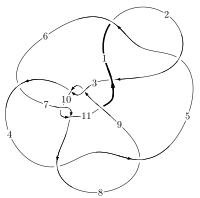
\includegraphics[width=112pt]{../../../GIT/diagram.site/Diagrams/png/406_11a_157.png}\\
\ \ \ A knot diagram\footnotemark}&
\allowdisplaybreaks
\textbf{Linearized knot diagam} \\
\cline{2-2}
 &
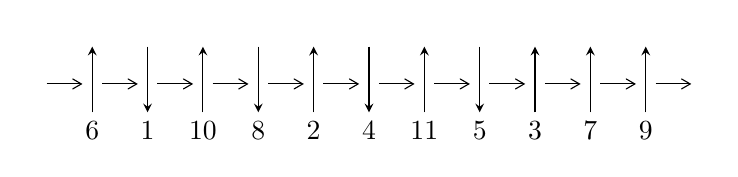
\begin{tikzpicture}[x=20pt, y=17pt]
	% nodes
	\node (C0) at (0, 0) {};
	\node (C1) at (1, 0) {};
	\node (C1U) at (1, +1) {};
	\node (C1D) at (1, -1) {6};

	\node (C2) at (2, 0) {};
	\node (C2U) at (2, +1) {};
	\node (C2D) at (2, -1) {1};

	\node (C3) at (3, 0) {};
	\node (C3U) at (3, +1) {};
	\node (C3D) at (3, -1) {10};

	\node (C4) at (4, 0) {};
	\node (C4U) at (4, +1) {};
	\node (C4D) at (4, -1) {8};

	\node (C5) at (5, 0) {};
	\node (C5U) at (5, +1) {};
	\node (C5D) at (5, -1) {2};

	\node (C6) at (6, 0) {};
	\node (C6U) at (6, +1) {};
	\node (C6D) at (6, -1) {4};

	\node (C7) at (7, 0) {};
	\node (C7U) at (7, +1) {};
	\node (C7D) at (7, -1) {11};

	\node (C8) at (8, 0) {};
	\node (C8U) at (8, +1) {};
	\node (C8D) at (8, -1) {5};

	\node (C9) at (9, 0) {};
	\node (C9U) at (9, +1) {};
	\node (C9D) at (9, -1) {3};

	\node (C10) at (10, 0) {};
	\node (C10U) at (10, +1) {};
	\node (C10D) at (10, -1) {7};

	\node (C11) at (11, 0) {};
	\node (C11U) at (11, +1) {};
	\node (C11D) at (11, -1) {9};
	\node (C12) at (12, 0) {};

	% arrows
	\draw[->,>={angle 60}]
	(C0) edge (C1) (C1) edge (C2) (C2) edge (C3) (C3) edge (C4) (C4) edge (C5) (C5) edge (C6) (C6) edge (C7) (C7) edge (C8) (C8) edge (C9) (C9) edge (C10) (C10) edge (C11) (C11) edge (C12) ;	\draw[->,>=stealth]
	(C1D) edge (C1U) (C2U) edge (C2D) (C3D) edge (C3U) (C4U) edge (C4D) (C5D) edge (C5U) (C6U) edge (C6D) (C7D) edge (C7U) (C8U) edge (C8D) (C9D) edge (C9U) (C10D) edge (C10U) (C11D) edge (C11U) ;
	\end{tikzpicture} \\
\hhline{~~} \\& 
\textbf{Solving Sequence} \\ \cline{2-2} 
 &
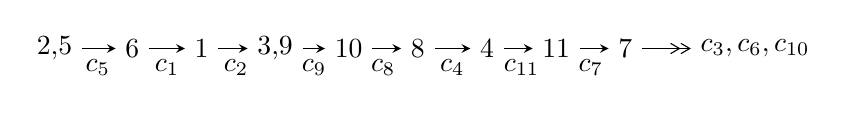
\begin{tikzpicture}[x=25pt, y=7pt]
	% node
	\node (A0) at (-1/8, 0) {2,5};
	\node (A1) at (1, 0) {6};
	\node (A2) at (2, 0) {1};
	\node (A3) at (49/16, 0) {3,9};
	\node (A4) at (33/8, 0) {10};
	\node (A5) at (41/8, 0) {8};
	\node (A6) at (49/8, 0) {4};
	\node (A7) at (57/8, 0) {11};
	\node (A8) at (65/8, 0) {7};
	\node (C1) at (1/2, -1) {$c_{5}$};
	\node (C2) at (3/2, -1) {$c_{1}$};
	\node (C3) at (5/2, -1) {$c_{2}$};
	\node (C4) at (29/8, -1) {$c_{9}$};
	\node (C5) at (37/8, -1) {$c_{8}$};
	\node (C6) at (45/8, -1) {$c_{4}$};
	\node (C7) at (53/8, -1) {$c_{11}$};
	\node (C8) at (61/8, -1) {$c_{7}$};
	\node (A9) at (10, 0) {$c_{3},c_{6},c_{10}$};

	% edge
	\draw[->,>=stealth]	
	(A0) edge (A1) (A1) edge (A2) (A2) edge (A3) (A3) edge (A4) (A4) edge (A5) (A5) edge (A6) (A6) edge (A7) (A7) edge (A8) ;
	\draw[->>,>={angle 60}]	
	(A8) edge (A9);
\end{tikzpicture} \\ 

\end{tabular} \\

\footnotetext{
The image of knot diagram is generated by the software ``\textbf{Draw programme}" developed by Andrew Bartholomew(\url{http://www.layer8.co.uk/maths/draw/index.htm\#Running-draw}), where we modified some parts for our purpose(\url{https://github.com/CATsTAILs/LinksPainter}).
}\phantom \\ \newline 
\centering \textbf{Ideals for irreducible components\footnotemark of $X_{\text{par}}$} 
 
\begin{align*}
I^u_{1}&=\langle 
-116 u^{51}-310 u^{50}+\cdots+2304 b+7136,\;-3775 u^{52}-16066 u^{51}+\cdots+52992 a+229724,\\
\phantom{I^u_{1}}&\phantom{= \langle  }u^{53}+4 u^{52}+\cdots-92 u-46\rangle \\
I^u_{2}&=\langle 
- a^2 u+2 b+a-2,\;a^3+2 a^2 u- a u+2 a+2,\;u^2- u+1\rangle \\
I^u_{3}&=\langle 
b+1,\;6 a+u+4,\;u^2+2\rangle \\
I^u_{4}&=\langle 
b^2 a u+b^3- b u- a u- b+u-1,\;u^2- u+1\rangle \\
\\
I^v_{1}&=\langle 
a,\;b^3- b-1,\;v-1\rangle \\
I^v_{2}&=\langle 
a,\;b-1,\;v-1\rangle \\
\end{align*}
\raggedright * 5 irreducible components of $\dim_{\mathbb{C}}=0$, with total 65 representations.\\
\raggedright * 1 irreducible components of $\dim_{\mathbb{C}}=1$ \\
\footnotetext{All coefficients of polynomials are rational numbers. But the coefficients are sometimes approximated in decimal forms when there is not enough margin.}
\newpage
\renewcommand{\arraystretch}{1}
\centering \section*{I. $I^u_{1}= \langle -116 u^{51}-310 u^{50}+\cdots+2304 b+7136,\;-3775 u^{52}-16066 u^{51}+\cdots+52992 a+229724,\;u^{53}+4 u^{52}+\cdots-92 u-46 \rangle$}
\flushleft \textbf{(i) Arc colorings}\\
\begin{tabular}{m{7pt} m{180pt} m{7pt} m{180pt} }
\flushright $a_{2}=$&$\begin{pmatrix}0\\u\end{pmatrix}$ \\
\flushright $a_{5}=$&$\begin{pmatrix}1\\0\end{pmatrix}$ \\
\flushright $a_{6}=$&$\begin{pmatrix}1\\- u^2\end{pmatrix}$ \\
\flushright $a_{1}=$&$\begin{pmatrix}- u\\u^3+u\end{pmatrix}$ \\
\flushright $a_{3}=$&$\begin{pmatrix}- u^3\\u^5+u^3+u\end{pmatrix}$ \\
\flushright $a_{9}=$&$\begin{pmatrix}0.0712372 u^{52}+0.303178 u^{51}+\cdots-8.73049 u-4.33507\\0.0503472 u^{51}+0.134549 u^{50}+\cdots-1.31510 u-3.09722\end{pmatrix}$ \\
\flushright $a_{10}=$&$\begin{pmatrix}0.184518 u^{52}+0.705088 u^{51}+\cdots-14.9597 u-6.29167\\0.0625000 u^{52}+0.159722 u^{51}+\cdots-1.55729 u-1.65972\end{pmatrix}$ \\
\flushright $a_{8}=$&$\begin{pmatrix}0.0712372 u^{52}+0.353525 u^{51}+\cdots-10.0456 u-7.43229\\0.0503472 u^{51}+0.134549 u^{50}+\cdots-1.31510 u-3.09722\end{pmatrix}$ \\
\flushright $a_{4}=$&$\begin{pmatrix}0.119226 u^{52}+0.443048 u^{51}+\cdots-9.10745 u-4.01302\\0.00520833 u^{52}-0.0195313 u^{51}+\cdots+1.50521 u+0.684896\end{pmatrix}$ \\
\flushright $a_{11}=$&$\begin{pmatrix}-0.0306839 u^{52}-0.0914855 u^{51}+\cdots+4.15433 u+4.34635\\0.109375 u^{52}+0.342448 u^{51}+\cdots-4.84375 u-0.565104\end{pmatrix}$ \\
\flushright $a_{7}=$&$\begin{pmatrix}-0.0805405 u^{52}-0.300460 u^{51}+\cdots+7.03842 u+4.68750\\-0.0625000 u^{52}-0.165799 u^{51}+\cdots+0.802083 u+1.18924\end{pmatrix}$\\ \flushright $a_{7}=$&$\begin{pmatrix}-0.0805405 u^{52}-0.300460 u^{51}+\cdots+7.03842 u+4.68750\\-0.0625000 u^{52}-0.165799 u^{51}+\cdots+0.802083 u+1.18924\end{pmatrix}$\\&\end{tabular}
\flushleft \textbf{(ii) Obstruction class $= -1$}\\~\\
\flushleft \textbf{(iii) Cusp Shapes $= \frac{1153}{1728} u^{52}+\frac{1951}{864} u^{51}+\cdots-\frac{7271}{216} u+\frac{1}{4}$}\\~\\
\newpage\renewcommand{\arraystretch}{1}
\flushleft \textbf{(iv) u-Polynomials at the component}\newline \\
\begin{tabular}{m{50pt}|m{274pt}}
Crossings & \hspace{64pt}u-Polynomials at each crossing \\
\hline $$\begin{aligned}c_{1},c_{5}\end{aligned}$$&$\begin{aligned}
&u^{53}+4 u^{52}+\cdots-92 u-46
\end{aligned}$\\
\hline $$\begin{aligned}c_{2}\end{aligned}$$&$\begin{aligned}
&u^{53}+24 u^{52}+\cdots+3496 u-2116
\end{aligned}$\\
\hline $$\begin{aligned}c_{3},c_{9}\end{aligned}$$&$\begin{aligned}
&9(9 u^{53}-18 u^{52}+\cdots-77 u-19)
\end{aligned}$\\
\hline $$\begin{aligned}c_{4},c_{8}\end{aligned}$$&$\begin{aligned}
&9(9 u^{53}+18 u^{52}+\cdots-9 u-19)
\end{aligned}$\\
\hline $$\begin{aligned}c_{6}\end{aligned}$$&$\begin{aligned}
&16(16 u^{53}-16 u^{52}+\cdots+103779 u-3609)
\end{aligned}$\\
\hline $$\begin{aligned}c_{7},c_{10}\end{aligned}$$&$\begin{aligned}
&u^{53}+6 u^{52}+\cdots-5832 u-1706
\end{aligned}$\\
\hline $$\begin{aligned}c_{11}\end{aligned}$$&$\begin{aligned}
&16(16 u^{53}+32 u^{52}+\cdots-16641 u-6003)
\end{aligned}$\\
\hline
\end{tabular}\\~\\
\newpage\renewcommand{\arraystretch}{1}
\flushleft \textbf{(v) Riley Polynomials at the component}\newline \\
\begin{tabular}{m{50pt}|m{274pt}}
Crossings & \hspace{64pt}Riley Polynomials at each crossing \\
\hline $$\begin{aligned}c_{1},c_{5}\end{aligned}$$&$\begin{aligned}
&y^{53}+24 y^{52}+\cdots+3496 y-2116
\end{aligned}$\\
\hline $$\begin{aligned}c_{2}\end{aligned}$$&$\begin{aligned}
&y^{53}+12 y^{52}+\cdots+393508288 y-4477456
\end{aligned}$\\
\hline $$\begin{aligned}c_{3},c_{9}\end{aligned}$$&$\begin{aligned}
&81(81 y^{53}-3510 y^{52}+\cdots+3421 y-361)
\end{aligned}$\\
\hline $$\begin{aligned}c_{4},c_{8}\end{aligned}$$&$\begin{aligned}
&81(81 y^{53}-2214 y^{52}+\cdots+7149 y-361)
\end{aligned}$\\
\hline $$\begin{aligned}c_{6}\end{aligned}$$&$\begin{aligned}
&256(256 y^{53}+6016 y^{52}+\cdots+9.94255\times10^{9} y-1.30249\times10^{7})
\end{aligned}$\\
\hline $$\begin{aligned}c_{7},c_{10}\end{aligned}$$&$\begin{aligned}
&y^{53}-30 y^{52}+\cdots-5573800 y-2910436
\end{aligned}$\\
\hline $$\begin{aligned}c_{11}\end{aligned}$$&$\begin{aligned}
&256(256 y^{53}-6528 y^{52}+\cdots-3.68087\times10^{8} y-3.60360\times10^{7})
\end{aligned}$\\
\hline
\end{tabular}\\~\\
\newpage\flushleft \textbf{(vi) Complex Volumes and Cusp Shapes}
$$\begin{array}{c|c|c}  
\text{Solutions to }I^u_{1}& \I (\text{vol} + \sqrt{-1}CS) & \text{Cusp shape}\\
 \hline 
\begin{aligned}
u &= -0.809668 + 0.591571 I \\
a &= -0.38862 + 1.53061 I \\
b &= -0.262654 - 1.151540 I\end{aligned}
 & \phantom{-}9.44289 + 4.62072 I & \phantom{-}10.24286 - 2.08237 I \\ \hline\begin{aligned}
u &= -0.809668 - 0.591571 I \\
a &= -0.38862 - 1.53061 I \\
b &= -0.262654 + 1.151540 I\end{aligned}
 & \phantom{-}9.44289 - 4.62072 I & \phantom{-}10.24286 + 2.08237 I \\ \hline\begin{aligned}
u &= \phantom{-}0.932904 + 0.475451 I \\
a &= \phantom{-}0.719049 + 0.844934 I \\
b &= -1.26960 - 0.64309 I\end{aligned}
 & \phantom{-}6.27152 - 10.90750 I & \phantom{-}7.14898 + 5.53843 I \\ \hline\begin{aligned}
u &= \phantom{-}0.932904 - 0.475451 I \\
a &= \phantom{-}0.719049 - 0.844934 I \\
b &= -1.26960 + 0.64309 I\end{aligned}
 & \phantom{-}6.27152 + 10.90750 I & \phantom{-}7.14898 - 5.53843 I \\ \hline\begin{aligned}
u &= \phantom{-}0.880838 + 0.326928 I \\
a &= -0.164167 + 0.799269 I \\
b &= -0.573186 - 0.653434 I\end{aligned}
 & \phantom{-}7.95194 + 1.12051 I & \phantom{-}10.90095 + 0.04798 I \\ \hline\begin{aligned}
u &= \phantom{-}0.880838 - 0.326928 I \\
a &= -0.164167 - 0.799269 I \\
b &= -0.573186 + 0.653434 I\end{aligned}
 & \phantom{-}7.95194 - 1.12051 I & \phantom{-}10.90095 - 0.04798 I \\ \hline\begin{aligned}
u &= -0.817792 + 0.679811 I \\
a &= \phantom{-}0.418946 - 0.981125 I \\
b &= \phantom{-}0.303446 + 0.604240 I\end{aligned}
 & \phantom{-}4.38963 + 0.38285 I & \phantom{-}8.33080 + 0.50210 I \\ \hline\begin{aligned}
u &= -0.817792 - 0.679811 I \\
a &= \phantom{-}0.418946 + 0.981125 I \\
b &= \phantom{-}0.303446 - 0.604240 I\end{aligned}
 & \phantom{-}4.38963 - 0.38285 I & \phantom{-}8.33080 - 0.50210 I \\ \hline\begin{aligned}
u &= \phantom{-}0.994126 + 0.446360 I \\
a &= -0.477878 - 0.579642 I \\
b &= \phantom{-}1.071810 + 0.473560 I\end{aligned}
 & \phantom{-}2.22320 - 4.60694 I & \phantom{-}5.52820 + 4.35998 I \\ \hline\begin{aligned}
u &= \phantom{-}0.994126 - 0.446360 I \\
a &= -0.477878 + 0.579642 I \\
b &= \phantom{-}1.071810 - 0.473560 I\end{aligned}
 & \phantom{-}2.22320 + 4.60694 I & \phantom{-}5.52820 - 4.35998 I\\
 \hline 
 \end{array}$$\newpage$$\begin{array}{c|c|c}  
\text{Solutions to }I^u_{1}& \I (\text{vol} + \sqrt{-1}CS) & \text{Cusp shape}\\
 \hline 
\begin{aligned}
u &= \phantom{-}0.611609 + 0.908410 I \\
a &= -1.30709 + 0.63481 I \\
b &= \phantom{-}0.809891 + 0.174593 I\end{aligned}
 & \phantom{-}0.872134 + 1.079720 I & \phantom{-0.000000 -}0. + 2.41019 I \\ \hline\begin{aligned}
u &= \phantom{-}0.611609 - 0.908410 I \\
a &= -1.30709 - 0.63481 I \\
b &= \phantom{-}0.809891 - 0.174593 I\end{aligned}
 & \phantom{-}0.872134 - 1.079720 I & \phantom{-0.000000 } 0. - 2.41019 I \\ \hline\begin{aligned}
u &= \phantom{-}0.170302 + 1.087830 I \\
a &= \phantom{-}0.635126 + 0.069933 I \\
b &= \phantom{-}0.001690 + 0.649953 I\end{aligned}
 & \phantom{-}3.08054 + 4.00121 I & \phantom{-}5.97068 - 4.06106 I \\ \hline\begin{aligned}
u &= \phantom{-}0.170302 - 1.087830 I \\
a &= \phantom{-}0.635126 - 0.069933 I \\
b &= \phantom{-}0.001690 - 0.649953 I\end{aligned}
 & \phantom{-}3.08054 - 4.00121 I & \phantom{-}5.97068 + 4.06106 I \\ \hline\begin{aligned}
u &= \phantom{-}0.626566 + 0.643943 I \\
a &= \phantom{-}1.22653 - 0.71815 I \\
b &= -0.826327 + 0.364980 I\end{aligned}
 & \phantom{-}1.59094 + 3.76796 I & \phantom{-}4.39825 - 7.64009 I \\ \hline\begin{aligned}
u &= \phantom{-}0.626566 - 0.643943 I \\
a &= \phantom{-}1.22653 + 0.71815 I \\
b &= -0.826327 - 0.364980 I\end{aligned}
 & \phantom{-}1.59094 - 3.76796 I & \phantom{-}4.39825 + 7.64009 I \\ \hline\begin{aligned}
u &= -0.128610 + 1.112310 I \\
a &= \phantom{-}0.653956 - 0.300609 I \\
b &= \phantom{-}1.275160 - 0.403466 I\end{aligned}
 & -4.15345 + 3.73758 I & -2.48655 - 3.09856 I \\ \hline\begin{aligned}
u &= -0.128610 - 1.112310 I \\
a &= \phantom{-}0.653956 + 0.300609 I \\
b &= \phantom{-}1.275160 + 0.403466 I\end{aligned}
 & -4.15345 - 3.73758 I & -2.48655 + 3.09856 I \\ \hline\begin{aligned}
u &= -0.949759 + 0.608985 I \\
a &= \phantom{-}0.264387 + 0.875055 I \\
b &= -0.908688 - 0.564102 I\end{aligned}
 & \phantom{-}6.99581 - 5.82913 I & \phantom{-}8.82739 + 6.38685 I \\ \hline\begin{aligned}
u &= -0.949759 - 0.608985 I \\
a &= \phantom{-}0.264387 - 0.875055 I \\
b &= -0.908688 + 0.564102 I\end{aligned}
 & \phantom{-}6.99581 + 5.82913 I & \phantom{-}8.82739 - 6.38685 I\\
 \hline 
 \end{array}$$\newpage$$\begin{array}{c|c|c}  
\text{Solutions to }I^u_{1}& \I (\text{vol} + \sqrt{-1}CS) & \text{Cusp shape}\\
 \hline 
\begin{aligned}
u &= -0.496009 + 1.017750 I \\
a &= \phantom{-}1.36846 - 1.83838 I \\
b &= \phantom{-}0.878140 + 0.204929 I\end{aligned}
 & \phantom{-}0.67079 - 3.09135 I & \phantom{-0.000000 -}0. + 5.67301 I \\ \hline\begin{aligned}
u &= -0.496009 - 1.017750 I \\
a &= \phantom{-}1.36846 + 1.83838 I \\
b &= \phantom{-}0.878140 - 0.204929 I\end{aligned}
 & \phantom{-}0.67079 + 3.09135 I & \phantom{-0.000000 } 0. - 5.67301 I \\ \hline\begin{aligned}
u &= -0.724250 + 0.436534 I \\
a &= \phantom{-}1.15534 - 0.92210 I \\
b &= -1.151270 + 0.693551 I\end{aligned}
 & \phantom{-}0.72806 + 5.75739 I & \phantom{-}4.99130 - 5.10418 I \\ \hline\begin{aligned}
u &= -0.724250 - 0.436534 I \\
a &= \phantom{-}1.15534 + 0.92210 I \\
b &= -1.151270 - 0.693551 I\end{aligned}
 & \phantom{-}0.72806 - 5.75739 I & \phantom{-}4.99130 + 5.10418 I \\ \hline\begin{aligned}
u &= -0.434366 + 0.666743 I \\
a &= \phantom{-}0.33515 - 2.08440 I \\
b &= -0.607875 + 0.260312 I\end{aligned}
 & \phantom{-}1.88416 - 0.85038 I & \phantom{-}6.25673 - 3.20224 I \\ \hline\begin{aligned}
u &= -0.434366 - 0.666743 I \\
a &= \phantom{-}0.33515 + 2.08440 I \\
b &= -0.607875 - 0.260312 I\end{aligned}
 & \phantom{-}1.88416 + 0.85038 I & \phantom{-}6.25673 + 3.20224 I \\ \hline\begin{aligned}
u &= -0.212305 + 1.189430 I \\
a &= -0.778145 + 0.361047 I \\
b &= -1.237090 + 0.111866 I\end{aligned}
 & -6.51253 - 1.42478 I & \phantom{-0.000000 } 0 \\ \hline\begin{aligned}
u &= -0.212305 - 1.189430 I \\
a &= -0.778145 - 0.361047 I \\
b &= -1.237090 - 0.111866 I\end{aligned}
 & -6.51253 + 1.42478 I & \phantom{-0.000000 } 0 \\ \hline\begin{aligned}
u &= -0.686889 + 1.004730 I \\
a &= \phantom{-}0.343976 - 0.826525 I \\
b &= -0.085142 + 0.784336 I\end{aligned}
 & \phantom{-}3.37147 - 6.01200 I & \phantom{-0.000000 } 0 \\ \hline\begin{aligned}
u &= -0.686889 - 1.004730 I \\
a &= \phantom{-}0.343976 + 0.826525 I \\
b &= -0.085142 - 0.784336 I\end{aligned}
 & \phantom{-}3.37147 + 6.01200 I & \phantom{-0.000000 } 0\\
 \hline 
 \end{array}$$\newpage$$\begin{array}{c|c|c}  
\text{Solutions to }I^u_{1}& \I (\text{vol} + \sqrt{-1}CS) & \text{Cusp shape}\\
 \hline 
\begin{aligned}
u &= -0.572191 + 1.085580 I \\
a &= -0.52093 + 1.70529 I \\
b &= -1.240970 - 0.438253 I\end{aligned}
 & -4.09769 - 6.18849 I & \phantom{-0.000000 } 0 \\ \hline\begin{aligned}
u &= -0.572191 - 1.085580 I \\
a &= -0.52093 - 1.70529 I \\
b &= -1.240970 + 0.438253 I\end{aligned}
 & -4.09769 + 6.18849 I & \phantom{-0.000000 } 0 \\ \hline\begin{aligned}
u &= -0.601851 + 1.072670 I \\
a &= \phantom{-}0.51488 - 1.93050 I \\
b &= \phantom{-}1.31349 + 0.76096 I\end{aligned}
 & -1.10548 - 10.82140 I & \phantom{-0.000000 } 0 \\ \hline\begin{aligned}
u &= -0.601851 - 1.072670 I \\
a &= \phantom{-}0.51488 + 1.93050 I \\
b &= \phantom{-}1.31349 - 0.76096 I\end{aligned}
 & -1.10548 + 10.82140 I & \phantom{-0.000000 } 0 \\ \hline\begin{aligned}
u &= \phantom{-}0.055611 + 0.764069 I \\
a &= -0.284386 + 0.734524 I \\
b &= \phantom{-}0.575442 - 0.355913 I\end{aligned}
 & -1.00556 + 1.44727 I & -1.64819 - 5.47738 I \\ \hline\begin{aligned}
u &= \phantom{-}0.055611 - 0.764069 I \\
a &= -0.284386 - 0.734524 I \\
b &= \phantom{-}0.575442 + 0.355913 I\end{aligned}
 & -1.00556 - 1.44727 I & -1.64819 + 5.47738 I \\ \hline\begin{aligned}
u &= -0.673460 + 1.041740 I \\
a &= -0.955719 + 0.894786 I \\
b &= \phantom{-}0.132760 - 1.273430 I\end{aligned}
 & \phantom{-}8.08301 - 10.18320 I & \phantom{-0.000000 } 0 \\ \hline\begin{aligned}
u &= -0.673460 - 1.041740 I \\
a &= -0.955719 - 0.894786 I \\
b &= \phantom{-}0.132760 + 1.273430 I\end{aligned}
 & \phantom{-}8.08301 + 10.18320 I & \phantom{-0.000000 } 0 \\ \hline\begin{aligned}
u &= -0.681987 + 0.321709 I \\
a &= -0.724827 + 0.615572 I \\
b &= \phantom{-}1.078220 - 0.328843 I\end{aligned}
 & -1.99983 + 1.37832 I & -0.467710 - 0.890691 I \\ \hline\begin{aligned}
u &= -0.681987 - 0.321709 I \\
a &= -0.724827 - 0.615572 I \\
b &= \phantom{-}1.078220 + 0.328843 I\end{aligned}
 & -1.99983 - 1.37832 I & -0.467710 + 0.890691 I\\
 \hline 
 \end{array}$$\newpage$$\begin{array}{c|c|c}  
\text{Solutions to }I^u_{1}& \I (\text{vol} + \sqrt{-1}CS) & \text{Cusp shape}\\
 \hline 
\begin{aligned}
u &= -0.780684 + 1.053130 I \\
a &= -0.293135 - 0.040674 I \\
b &= \phantom{-}0.683599 - 0.489569 I\end{aligned}
 & \phantom{-}5.65031 - 0.44478 I & \phantom{-0.000000 } 0 \\ \hline\begin{aligned}
u &= -0.780684 - 1.053130 I \\
a &= -0.293135 + 0.040674 I \\
b &= \phantom{-}0.683599 + 0.489569 I\end{aligned}
 & \phantom{-}5.65031 + 0.44478 I & \phantom{-0.000000 } 0 \\ \hline\begin{aligned}
u &= \phantom{-}0.013214 + 1.311610 I \\
a &= \phantom{-}0.807998 - 0.074133 I \\
b &= \phantom{-}1.204730 + 0.451072 I\end{aligned}
 & -0.35444 - 8.20749 I & \phantom{-0.000000 } 0 \\ \hline\begin{aligned}
u &= \phantom{-}0.013214 - 1.311610 I \\
a &= \phantom{-}0.807998 + 0.074133 I \\
b &= \phantom{-}1.204730 - 0.451072 I\end{aligned}
 & -0.35444 + 8.20749 I & \phantom{-0.000000 } 0 \\ \hline\begin{aligned}
u &= \phantom{-}0.680239 + 1.136940 I \\
a &= \phantom{-}0.55415 + 1.83786 I \\
b &= \phantom{-}1.35544 - 0.64421 I\end{aligned}
 & \phantom{-}4.2476 + 16.8128 I & \phantom{-0.000000 } 0 \\ \hline\begin{aligned}
u &= \phantom{-}0.680239 - 1.136940 I \\
a &= \phantom{-}0.55415 - 1.83786 I \\
b &= \phantom{-}1.35544 + 0.64421 I\end{aligned}
 & \phantom{-}4.2476 - 16.8128 I & \phantom{-0.000000 } 0 \\ \hline\begin{aligned}
u &= \phantom{-}0.695044 + 1.161580 I \\
a &= -0.43161 - 1.48086 I \\
b &= -1.215140 + 0.489831 I\end{aligned}
 & \phantom{-}0.03277 + 10.71240 I & \phantom{-0.000000 } 0 \\ \hline\begin{aligned}
u &= \phantom{-}0.695044 - 1.161580 I \\
a &= -0.43161 + 1.48086 I \\
b &= -1.215140 - 0.489831 I\end{aligned}
 & \phantom{-}0.03277 - 10.71240 I & \phantom{-0.000000 } 0 \\ \hline\begin{aligned}
u &= \phantom{-}0.621820 + 1.215440 I \\
a &= \phantom{-}0.821143 + 0.925875 I \\
b &= \phantom{-}0.823061 - 0.470093 I\end{aligned}
 & \phantom{-}5.26202 + 4.45797 I & \phantom{-0.000000 } 0 \\ \hline\begin{aligned}
u &= \phantom{-}0.621820 - 1.215440 I \\
a &= \phantom{-}0.821143 - 0.925875 I \\
b &= \phantom{-}0.823061 + 0.470093 I\end{aligned}
 & \phantom{-}5.26202 - 4.45797 I & \phantom{-0.000000 } 0\\
 \hline 
 \end{array}$$\newpage$$\begin{array}{c|c|c}  
\text{Solutions to }I^u_{1}& \I (\text{vol} + \sqrt{-1}CS) & \text{Cusp shape}\\
 \hline 
\begin{aligned}
u &= \phantom{-}0.12822 + 1.49963 I \\
a &= -0.590311 - 0.032839 I \\
b &= -0.946332 - 0.195707 I\end{aligned}
 & -4.67412 - 0.82373 I & \phantom{-0.000000 } 0 \\ \hline\begin{aligned}
u &= \phantom{-}0.12822 - 1.49963 I \\
a &= -0.590311 + 0.032839 I \\
b &= -0.946332 + 0.195707 I\end{aligned}
 & -4.67412 + 0.82373 I & \phantom{-0.000000 } 0 \\ \hline\begin{aligned}
u &= \phantom{-}0.318662\phantom{ +0.000000I} \\
a &= \phantom{-}2.19545\phantom{ +0.000000I} \\
b &= -0.365228\phantom{ +0.000000I}\end{aligned}
 & \phantom{-}1.00464\phantom{ +0.000000I} & \phantom{-}11.4100\phantom{ +0.000000I}\\
 \hline 
 \end{array}$$\newpage\newpage\renewcommand{\arraystretch}{1}
\centering \section*{II. $I^u_{2}= \langle - a^2 u+2 b+a-2,\;a^3+2 a^2 u- a u+2 a+2,\;u^2- u+1 \rangle$}
\flushleft \textbf{(i) Arc colorings}\\
\begin{tabular}{m{7pt} m{180pt} m{7pt} m{180pt} }
\flushright $a_{2}=$&$\begin{pmatrix}0\\u\end{pmatrix}$ \\
\flushright $a_{5}=$&$\begin{pmatrix}1\\0\end{pmatrix}$ \\
\flushright $a_{6}=$&$\begin{pmatrix}1\\- u+1\end{pmatrix}$ \\
\flushright $a_{1}=$&$\begin{pmatrix}- u\\u-1\end{pmatrix}$ \\
\flushright $a_{3}=$&$\begin{pmatrix}1\\0\end{pmatrix}$ \\
\flushright $a_{9}=$&$\begin{pmatrix}a\\\frac{1}{2} a^2 u-\frac{1}{2} a+1\end{pmatrix}$ \\
\flushright $a_{10}=$&$\begin{pmatrix}\frac{1}{2} a^2 u+\frac{1}{2} a+1\\\frac{1}{2} a^2 u-\frac{1}{2} a+1\end{pmatrix}$ \\
\flushright $a_{8}=$&$\begin{pmatrix}\frac{1}{2} a^2 u+\frac{1}{2} a+1\\\frac{1}{2} a^2 u-\frac{1}{2} a+1\end{pmatrix}$ \\
\flushright $a_{4}=$&$\begin{pmatrix}\frac{1}{2} a^2 u+\frac{1}{2} a+1\\-\frac{1}{2} a^2 u+\frac{1}{2} a^2-\frac{1}{2} a u+a- u\end{pmatrix}$ \\
\flushright $a_{11}=$&$\begin{pmatrix}-\frac{1}{2} a^2 u-\frac{1}{2} a-1\\-\frac{1}{2} a^2 u+\frac{1}{2} a-1\end{pmatrix}$ \\
\flushright $a_{7}=$&$\begin{pmatrix}\frac{1}{2} a^2 u+\frac{1}{2} a+1\\\frac{1}{2} a^2 u-\frac{1}{2} a+1\end{pmatrix}$\\ \flushright $a_{7}=$&$\begin{pmatrix}\frac{1}{2} a^2 u+\frac{1}{2} a+1\\\frac{1}{2} a^2 u-\frac{1}{2} a+1\end{pmatrix}$\\&\end{tabular}
\flushleft \textbf{(ii) Obstruction class $= -1$}\\~\\
\flushleft \textbf{(iii) Cusp Shapes $= -4 u+2$}\\~\\
\newpage\renewcommand{\arraystretch}{1}
\flushleft \textbf{(iv) u-Polynomials at the component}\newline \\
\begin{tabular}{m{50pt}|m{274pt}}
Crossings & \hspace{64pt}u-Polynomials at each crossing \\
\hline $$\begin{aligned}c_{1},c_{5}\end{aligned}$$&$\begin{aligned}
&(u^2- u+1)^3
\end{aligned}$\\
\hline $$\begin{aligned}c_{2}\end{aligned}$$&$\begin{aligned}
&(u^2+u+1)^3
\end{aligned}$\\
\hline $$\begin{aligned}c_{3},c_{4},c_{6}\\c_{8},c_{9}\end{aligned}$$&$\begin{aligned}
&u^6-2 u^4- u^3+u^2+u+1
\end{aligned}$\\
\hline $$\begin{aligned}c_{7},c_{10}\end{aligned}$$&$\begin{aligned}
&u^6
\end{aligned}$\\
\hline $$\begin{aligned}c_{11}\end{aligned}$$&$\begin{aligned}
&u^6-4 u^5+6 u^4-3 u^3- u^2+u+1
\end{aligned}$\\
\hline
\end{tabular}\\~\\
\newpage\renewcommand{\arraystretch}{1}
\flushleft \textbf{(v) Riley Polynomials at the component}\newline \\
\begin{tabular}{m{50pt}|m{274pt}}
Crossings & \hspace{64pt}Riley Polynomials at each crossing \\
\hline $$\begin{aligned}c_{1},c_{2},c_{5}\end{aligned}$$&$\begin{aligned}
&(y^2+y+1)^3
\end{aligned}$\\
\hline $$\begin{aligned}c_{3},c_{4},c_{6}\\c_{8},c_{9}\end{aligned}$$&$\begin{aligned}
&y^6-4 y^5+6 y^4-3 y^3- y^2+y+1
\end{aligned}$\\
\hline $$\begin{aligned}c_{7},c_{10}\end{aligned}$$&$\begin{aligned}
&y^6
\end{aligned}$\\
\hline $$\begin{aligned}c_{11}\end{aligned}$$&$\begin{aligned}
&y^6-4 y^5+10 y^4-11 y^3+19 y^2-3 y+1
\end{aligned}$\\
\hline
\end{tabular}\\~\\
\newpage\flushleft \textbf{(vi) Complex Volumes and Cusp Shapes}
$$\begin{array}{c|c|c}  
\text{Solutions to }I^u_{2}& \I (\text{vol} + \sqrt{-1}CS) & \text{Cusp shape}\\
 \hline 
\begin{aligned}
u &= \phantom{-}0.500000 + 0.866025 I \\
a &= \phantom{-}0.412728 + 1.011420 I \\
b &= \phantom{-}0.218964 - 0.666188 I\end{aligned}
 & \phantom{-0.000000 -}2.02988 I & \phantom{-0.000000 } 0. - 3.46410 I \\ \hline\begin{aligned}
u &= \phantom{-}0.500000 + 0.866025 I \\
a &= -0.562490 - 0.528127 I \\
b &= \phantom{-}1.033350 + 0.428825 I\end{aligned}
 & \phantom{-0.000000 -}2.02988 I & \phantom{-0.000000 } 0. - 3.46410 I \\ \hline\begin{aligned}
u &= \phantom{-}0.500000 + 0.866025 I \\
a &= -0.85024 - 2.21534 I \\
b &= -1.252310 + 0.237364 I\end{aligned}
 & \phantom{-0.000000 -}2.02988 I & \phantom{-0.000000 } 0. - 3.46410 I \\ \hline\begin{aligned}
u &= \phantom{-}0.500000 - 0.866025 I \\
a &= \phantom{-}0.412728 - 1.011420 I \\
b &= \phantom{-}0.218964 + 0.666188 I\end{aligned}
 & \phantom{-0.000000 } -2.02988 I & \phantom{-0.000000 -}0. + 3.46410 I \\ \hline\begin{aligned}
u &= \phantom{-}0.500000 - 0.866025 I \\
a &= -0.562490 + 0.528127 I \\
b &= \phantom{-}1.033350 - 0.428825 I\end{aligned}
 & \phantom{-0.000000 } -2.02988 I & \phantom{-0.000000 -}0. + 3.46410 I \\ \hline\begin{aligned}
u &= \phantom{-}0.500000 - 0.866025 I \\
a &= -0.85024 + 2.21534 I \\
b &= -1.252310 - 0.237364 I\end{aligned}
 & \phantom{-0.000000 } -2.02988 I & \phantom{-0.000000 -}0. + 3.46410 I\\
 \hline 
 \end{array}$$\newpage\newpage\renewcommand{\arraystretch}{1}
\centering \section*{III. $I^u_{3}= \langle b+1,\;6 a+u+4,\;u^2+2 \rangle$}
\flushleft \textbf{(i) Arc colorings}\\
\begin{tabular}{m{7pt} m{180pt} m{7pt} m{180pt} }
\flushright $a_{2}=$&$\begin{pmatrix}0\\u\end{pmatrix}$ \\
\flushright $a_{5}=$&$\begin{pmatrix}1\\0\end{pmatrix}$ \\
\flushright $a_{6}=$&$\begin{pmatrix}1\\2\end{pmatrix}$ \\
\flushright $a_{1}=$&$\begin{pmatrix}- u\\- u\end{pmatrix}$ \\
\flushright $a_{3}=$&$\begin{pmatrix}2 u\\3 u\end{pmatrix}$ \\
\flushright $a_{9}=$&$\begin{pmatrix}-\frac{1}{6} u-\frac{2}{3}\\-1\end{pmatrix}$ \\
\flushright $a_{10}=$&$\begin{pmatrix}-\frac{13}{6} u-\frac{2}{3}\\-3 u-1\end{pmatrix}$ \\
\flushright $a_{8}=$&$\begin{pmatrix}-\frac{1}{6} u-\frac{5}{3}\\-1\end{pmatrix}$ \\
\flushright $a_{4}=$&$\begin{pmatrix}-\frac{1}{6} u-\frac{2}{3}\\-1\end{pmatrix}$ \\
\flushright $a_{11}=$&$\begin{pmatrix}-\frac{23}{18} u-\frac{1}{9}\\-\frac{4}{3} u-\frac{1}{3}\end{pmatrix}$ \\
\flushright $a_{7}=$&$\begin{pmatrix}-\frac{5}{18} u+\frac{8}{9}\\-\frac{1}{3} u+\frac{5}{3}\end{pmatrix}$\\ \flushright $a_{7}=$&$\begin{pmatrix}-\frac{5}{18} u+\frac{8}{9}\\-\frac{1}{3} u+\frac{5}{3}\end{pmatrix}$\\&\end{tabular}
\flushleft \textbf{(ii) Obstruction class $= 1$}\\~\\
\flushleft \textbf{(iii) Cusp Shapes $= 0$}\\~\\
\newpage\renewcommand{\arraystretch}{1}
\flushleft \textbf{(iv) u-Polynomials at the component}\newline \\
\begin{tabular}{m{50pt}|m{274pt}}
Crossings & \hspace{64pt}u-Polynomials at each crossing \\
\hline $$\begin{aligned}c_{1},c_{5},c_{7}\\c_{10}\end{aligned}$$&$\begin{aligned}
&u^2+2
\end{aligned}$\\
\hline $$\begin{aligned}c_{2}\end{aligned}$$&$\begin{aligned}
&(u+2)^2
\end{aligned}$\\
\hline $$\begin{aligned}c_{3},c_{4}\end{aligned}$$&$\begin{aligned}
&(u+1)^2
\end{aligned}$\\
\hline $$\begin{aligned}c_{6},c_{11}\end{aligned}$$&$\begin{aligned}
&3(3 u^2-2 u+1)
\end{aligned}$\\
\hline $$\begin{aligned}c_{8},c_{9}\end{aligned}$$&$\begin{aligned}
&(u-1)^2
\end{aligned}$\\
\hline
\end{tabular}\\~\\
\newpage\renewcommand{\arraystretch}{1}
\flushleft \textbf{(v) Riley Polynomials at the component}\newline \\
\begin{tabular}{m{50pt}|m{274pt}}
Crossings & \hspace{64pt}Riley Polynomials at each crossing \\
\hline $$\begin{aligned}c_{1},c_{5},c_{7}\\c_{10}\end{aligned}$$&$\begin{aligned}
&(y+2)^2
\end{aligned}$\\
\hline $$\begin{aligned}c_{2}\end{aligned}$$&$\begin{aligned}
&(y-4)^2
\end{aligned}$\\
\hline $$\begin{aligned}c_{3},c_{4},c_{8}\\c_{9}\end{aligned}$$&$\begin{aligned}
&(y-1)^2
\end{aligned}$\\
\hline $$\begin{aligned}c_{6},c_{11}\end{aligned}$$&$\begin{aligned}
&9(9 y^2+2 y+1)
\end{aligned}$\\
\hline
\end{tabular}\\~\\
\newpage\flushleft \textbf{(vi) Complex Volumes and Cusp Shapes}
$$\begin{array}{c|c|c}  
\text{Solutions to }I^u_{3}& \I (\text{vol} + \sqrt{-1}CS) & \text{Cusp shape}\\
 \hline 
\begin{aligned}
u &= \phantom{-0.000000 -}1.414210 I \\
a &= -0.666667 - 0.235702 I \\
b &= -1.00000\phantom{ +0.000000I}\end{aligned}
 & -4.93480\phantom{ +0.000000I} & \phantom{-0.000000 } 0 \\ \hline\begin{aligned}
u &= \phantom{-0.000000 } -1.414210 I \\
a &= -0.666667 + 0.235702 I \\
b &= -1.00000\phantom{ +0.000000I}\end{aligned}
 & -4.93480\phantom{ +0.000000I} & \phantom{-0.000000 } 0\\
 \hline 
 \end{array}$$\newpage\newpage\renewcommand{\arraystretch}{1}
\centering \section*{IV. $I^u_{4}= \langle b^2 a u+b^3- b u- a u- b+u-1,\;u^2- u+1 \rangle$}
\flushleft \textbf{(i) Arc colorings}\\
\begin{tabular}{m{7pt} m{180pt} m{7pt} m{180pt} }
\flushright $a_{2}=$&$\begin{pmatrix}0\\u\end{pmatrix}$ \\
\flushright $a_{5}=$&$\begin{pmatrix}1\\0\end{pmatrix}$ \\
\flushright $a_{6}=$&$\begin{pmatrix}1\\- u+1\end{pmatrix}$ \\
\flushright $a_{1}=$&$\begin{pmatrix}- u\\u-1\end{pmatrix}$ \\
\flushright $a_{3}=$&$\begin{pmatrix}1\\0\end{pmatrix}$ \\
\flushright $a_{9}=$&$\begin{pmatrix}a\\b\end{pmatrix}$ \\
\flushright $a_{10}=$&$\begin{pmatrix}b+a\\b\end{pmatrix}$ \\
\flushright $a_{8}=$&$\begin{pmatrix}b+a\\b\end{pmatrix}$ \\
\flushright $a_{4}=$&$\begin{pmatrix}- b^2- b a+1\\- b^2\end{pmatrix}$ \\
\flushright $a_{11}=$&$\begin{pmatrix}- b a u- a^2 u+a^2- u\\- b^2 u- b a u+b a+u-1\end{pmatrix}$ \\
\flushright $a_{7}=$&$\begin{pmatrix}b a u+a^2 u- a^2+b+a+u\\b^2 u+b a u- b a+b- u+1\end{pmatrix}$\\ \flushright $a_{7}=$&$\begin{pmatrix}b a u+a^2 u- a^2+b+a+u\\b^2 u+b a u- b a+b- u+1\end{pmatrix}$\\&\end{tabular}
\flushleft \textbf{(ii) Obstruction class $= 1$}\\~\\
\flushleft \textbf{(iii) Cusp Shapes $= -4 u+8$}\\~\\
\flushleft \textbf{(iv) u-Polynomials at the component} : It cannot be defined for a positive dimension component.\\~\\
\flushleft \textbf{(v) Riley Polynomials at the component} : It cannot be defined for a positive dimension component.\\~\\
\newpage\flushleft \textbf{(iv) Complex Volumes and Cusp Shapes}
$$\begin{array}{c|c|c} 
\text{Solution to }I^u_{4}& \I (\text{vol} + \sqrt{-1}CS) & \text{Cusp shape}\\
 \hline 
\begin{aligned}
u &= \cdots \\
a &= \cdots \\
b &= \cdots\end{aligned}
 & \phantom{-}1.64493 - 2.02988 I & \phantom{-}6.00000 - 3.46410 I\\
 \hline 
 \end{array}
$$\newpage\renewcommand{\arraystretch}{1}
\centering \section*{V. $I^v_{1}= \langle a,\;b^3- b-1,\;v-1 \rangle$}
\flushleft \textbf{(i) Arc colorings}\\
\begin{tabular}{m{7pt} m{180pt} m{7pt} m{180pt} }
\flushright $a_{2}=$&$\begin{pmatrix}1\\0\end{pmatrix}$ \\
\flushright $a_{5}=$&$\begin{pmatrix}1\\0\end{pmatrix}$ \\
\flushright $a_{6}=$&$\begin{pmatrix}1\\0\end{pmatrix}$ \\
\flushright $a_{1}=$&$\begin{pmatrix}1\\0\end{pmatrix}$ \\
\flushright $a_{3}=$&$\begin{pmatrix}1\\0\end{pmatrix}$ \\
\flushright $a_{9}=$&$\begin{pmatrix}0\\b\end{pmatrix}$ \\
\flushright $a_{10}=$&$\begin{pmatrix}b\\b\end{pmatrix}$ \\
\flushright $a_{8}=$&$\begin{pmatrix}b\\b\end{pmatrix}$ \\
\flushright $a_{4}=$&$\begin{pmatrix}- b^2+1\\- b^2\end{pmatrix}$ \\
\flushright $a_{11}=$&$\begin{pmatrix}1\\b^2\end{pmatrix}$ \\
\flushright $a_{7}=$&$\begin{pmatrix}b+1\\b^2+b\end{pmatrix}$\\ \flushright $a_{7}=$&$\begin{pmatrix}b+1\\b^2+b\end{pmatrix}$\\&\end{tabular}
\flushleft \textbf{(ii) Obstruction class $= -1$}\\~\\
\flushleft \textbf{(iii) Cusp Shapes $= 6$}\\~\\
\newpage\renewcommand{\arraystretch}{1}
\flushleft \textbf{(iv) u-Polynomials at the component}\newline \\
\begin{tabular}{m{50pt}|m{274pt}}
Crossings & \hspace{64pt}u-Polynomials at each crossing \\
\hline $$\begin{aligned}c_{1},c_{2},c_{5}\end{aligned}$$&$\begin{aligned}
&u^3
\end{aligned}$\\
\hline $$\begin{aligned}c_{3},c_{4},c_{8}\\c_{9},c_{11}\end{aligned}$$&$\begin{aligned}
&u^3- u+1
\end{aligned}$\\
\hline $$\begin{aligned}c_{6}\end{aligned}$$&$\begin{aligned}
&u^3+2 u^2+u+1
\end{aligned}$\\
\hline $$\begin{aligned}c_{7},c_{10}\end{aligned}$$&$\begin{aligned}
&(u-1)^3
\end{aligned}$\\
\hline
\end{tabular}\\~\\
\newpage\renewcommand{\arraystretch}{1}
\flushleft \textbf{(v) Riley Polynomials at the component}\newline \\
\begin{tabular}{m{50pt}|m{274pt}}
Crossings & \hspace{64pt}Riley Polynomials at each crossing \\
\hline $$\begin{aligned}c_{1},c_{2},c_{5}\end{aligned}$$&$\begin{aligned}
&y^3
\end{aligned}$\\
\hline $$\begin{aligned}c_{3},c_{4},c_{8}\\c_{9},c_{11}\end{aligned}$$&$\begin{aligned}
&y^3-2 y^2+y-1
\end{aligned}$\\
\hline $$\begin{aligned}c_{6}\end{aligned}$$&$\begin{aligned}
&y^3-2 y^2-3 y-1
\end{aligned}$\\
\hline $$\begin{aligned}c_{7},c_{10}\end{aligned}$$&$\begin{aligned}
&(y-1)^3
\end{aligned}$\\
\hline
\end{tabular}\\~\\
\newpage\flushleft \textbf{(vi) Complex Volumes and Cusp Shapes}
$$\begin{array}{c|c|c}  
\text{Solutions to }I^v_{1}& \I (\text{vol} + \sqrt{-1}CS) & \text{Cusp shape}\\
 \hline 
\begin{aligned}
v &= \phantom{-}1.00000\phantom{ +0.000000I} \\
a &= \phantom{-0.000000 } 0 \\
b &= -0.662359 + 0.562280 I\end{aligned}
 & \phantom{-}1.64493\phantom{ +0.000000I} & \phantom{-}6.00000\phantom{ +0.000000I} \\ \hline\begin{aligned}
v &= \phantom{-}1.00000\phantom{ +0.000000I} \\
a &= \phantom{-0.000000 } 0 \\
b &= -0.662359 - 0.562280 I\end{aligned}
 & \phantom{-}1.64493\phantom{ +0.000000I} & \phantom{-}6.00000\phantom{ +0.000000I} \\ \hline\begin{aligned}
v &= \phantom{-}1.00000\phantom{ +0.000000I} \\
a &= \phantom{-0.000000 } 0 \\
b &= \phantom{-}1.32472\phantom{ +0.000000I}\end{aligned}
 & \phantom{-}1.64493\phantom{ +0.000000I} & \phantom{-}6.00000\phantom{ +0.000000I}\\
 \hline 
 \end{array}$$\newpage\newpage\renewcommand{\arraystretch}{1}
\centering \section*{VI. $I^v_{2}= \langle a,\;b-1,\;v-1 \rangle$}
\flushleft \textbf{(i) Arc colorings}\\
\begin{tabular}{m{7pt} m{180pt} m{7pt} m{180pt} }
\flushright $a_{2}=$&$\begin{pmatrix}1\\0\end{pmatrix}$ \\
\flushright $a_{5}=$&$\begin{pmatrix}1\\0\end{pmatrix}$ \\
\flushright $a_{6}=$&$\begin{pmatrix}1\\0\end{pmatrix}$ \\
\flushright $a_{1}=$&$\begin{pmatrix}1\\0\end{pmatrix}$ \\
\flushright $a_{3}=$&$\begin{pmatrix}1\\0\end{pmatrix}$ \\
\flushright $a_{9}=$&$\begin{pmatrix}0\\1\end{pmatrix}$ \\
\flushright $a_{10}=$&$\begin{pmatrix}1\\1\end{pmatrix}$ \\
\flushright $a_{8}=$&$\begin{pmatrix}1\\1\end{pmatrix}$ \\
\flushright $a_{4}=$&$\begin{pmatrix}0\\-1\end{pmatrix}$ \\
\flushright $a_{11}=$&$\begin{pmatrix}1\\1\end{pmatrix}$ \\
\flushright $a_{7}=$&$\begin{pmatrix}1\\1\end{pmatrix}$\\ \flushright $a_{7}=$&$\begin{pmatrix}1\\1\end{pmatrix}$\\&\end{tabular}
\flushleft \textbf{(ii) Obstruction class $= 1$}\\~\\
\flushleft \textbf{(iii) Cusp Shapes $= 0$}\\~\\
\newpage\renewcommand{\arraystretch}{1}
\flushleft \textbf{(iv) u-Polynomials at the component}\newline \\
\begin{tabular}{m{50pt}|m{274pt}}
Crossings & \hspace{64pt}u-Polynomials at each crossing \\
\hline $$\begin{aligned}c_{1},c_{2},c_{5}\\c_{7},c_{10}\end{aligned}$$&$\begin{aligned}
&u
\end{aligned}$\\
\hline $$\begin{aligned}c_{3},c_{4},c_{11}\end{aligned}$$&$\begin{aligned}
&u-1
\end{aligned}$\\
\hline $$\begin{aligned}c_{6},c_{8},c_{9}\end{aligned}$$&$\begin{aligned}
&u+1
\end{aligned}$\\
\hline
\end{tabular}\\~\\
\newpage\renewcommand{\arraystretch}{1}
\flushleft \textbf{(v) Riley Polynomials at the component}\newline \\
\begin{tabular}{m{50pt}|m{274pt}}
Crossings & \hspace{64pt}Riley Polynomials at each crossing \\
\hline $$\begin{aligned}c_{1},c_{2},c_{5}\\c_{7},c_{10}\end{aligned}$$&$\begin{aligned}
&y
\end{aligned}$\\
\hline $$\begin{aligned}c_{3},c_{4},c_{6}\\c_{8},c_{9},c_{11}\end{aligned}$$&$\begin{aligned}
&y-1
\end{aligned}$\\
\hline
\end{tabular}\\~\\
\newpage\flushleft \textbf{(vi) Complex Volumes and Cusp Shapes}
$$\begin{array}{c|c|c}  
\text{Solutions to }I^v_{2}& \I (\text{vol} + \sqrt{-1}CS) & \text{Cusp shape}\\
 \hline 
\begin{aligned}
v &= \phantom{-}1.00000\phantom{ +0.000000I} \\
a &= \phantom{-0.000000 } 0 \\
b &= \phantom{-}1.00000\phantom{ +0.000000I}\end{aligned}
 & \phantom{-0.000000 } 0 & \phantom{-0.000000 } 0\\
 \hline 
 \end{array}$$\newpage
\newpage\renewcommand{\arraystretch}{1}
\centering \section*{ VII. u-Polynomials}
\begin{tabular}{m{50pt}|m{274pt}}
Crossings & \hspace{64pt}u-Polynomials at each crossing \\
\hline $$\begin{aligned}c_{1},c_{5}\end{aligned}$$&$\begin{aligned}
&u^4(u^2+2)(u^2- u+1)^3(u^{53}+4 u^{52}+\cdots-92 u-46)
\end{aligned}$\\
\hline $$\begin{aligned}c_{2}\end{aligned}$$&$\begin{aligned}
&u^4(u+2)^2(u^2+u+1)^3(u^{53}+24 u^{52}+\cdots+3496 u-2116)
\end{aligned}$\\
\hline $$\begin{aligned}c_{3}\end{aligned}$$&$\begin{aligned}
&9(u-1)(u+1)^2(u^3- u+1)(u^6-2 u^4- u^3+u^2+u+1)\\
&\cdot(9 u^{53}-18 u^{52}+\cdots-77 u-19)
\end{aligned}$\\
\hline $$\begin{aligned}c_{4}\end{aligned}$$&$\begin{aligned}
&9(u-1)(u+1)^2(u^3- u+1)(u^6-2 u^4- u^3+u^2+u+1)\\
&\cdot(9 u^{53}+18 u^{52}+\cdots-9 u-19)
\end{aligned}$\\
\hline $$\begin{aligned}c_{6}\end{aligned}$$&$\begin{aligned}
&48(u+1)(3 u^2-2 u+1)(u^{3}+2 u^{2}+u+1)(u^{6}-2 u^{4}+\cdots+u+1)\\
&\cdot(16 u^{53}-16 u^{52}+\cdots+103779 u-3609)
\end{aligned}$\\
\hline $$\begin{aligned}c_{7},c_{10}\end{aligned}$$&$\begin{aligned}
&u^7(u-1)^3(u^2+2)(u^{53}+6 u^{52}+\cdots-5832 u-1706)
\end{aligned}$\\
\hline $$\begin{aligned}c_{8}\end{aligned}$$&$\begin{aligned}
&9(u-1)^2(u+1)(u^3- u+1)(u^6-2 u^4- u^3+u^2+u+1)\\
&\cdot(9 u^{53}+18 u^{52}+\cdots-9 u-19)
\end{aligned}$\\
\hline $$\begin{aligned}c_{9}\end{aligned}$$&$\begin{aligned}
&9(u-1)^2(u+1)(u^3- u+1)(u^6-2 u^4- u^3+u^2+u+1)\\
&\cdot(9 u^{53}-18 u^{52}+\cdots-77 u-19)
\end{aligned}$\\
\hline $$\begin{aligned}c_{11}\end{aligned}$$&$\begin{aligned}
&48(u-1)(3 u^2-2 u+1)(u^3- u+1)(u^{6}-4 u^{5}+\cdots+u+1)\\
&\cdot(16 u^{53}+32 u^{52}+\cdots-16641 u-6003)
\end{aligned}$\\
\hline
\end{tabular}\newpage\renewcommand{\arraystretch}{1}
\centering \section*{ VIII. Riley Polynomials}
\begin{tabular}{m{50pt}|m{274pt}}
Crossings & \hspace{64pt}Riley Polynomials at each crossing \\
\hline $$\begin{aligned}c_{1},c_{5}\end{aligned}$$&$\begin{aligned}
&y^4(y+2)^2(y^2+y+1)^3(y^{53}+24 y^{52}+\cdots+3496 y-2116)
\end{aligned}$\\
\hline $$\begin{aligned}c_{2}\end{aligned}$$&$\begin{aligned}
&y^4(y-4)^2(y^2+y+1)^3\\
&\cdot(y^{53}+12 y^{52}+\cdots+393508288 y-4477456)
\end{aligned}$\\
\hline $$\begin{aligned}c_{3},c_{9}\end{aligned}$$&$\begin{aligned}
&81(y-1)^3(y^3-2 y^2+y-1)(y^6-4 y^5+6 y^4-3 y^3- y^2+y+1)\\
&\cdot(81 y^{53}-3510 y^{52}+\cdots+3421 y-361)
\end{aligned}$\\
\hline $$\begin{aligned}c_{4},c_{8}\end{aligned}$$&$\begin{aligned}
&81(y-1)^3(y^3-2 y^2+y-1)(y^6-4 y^5+6 y^4-3 y^3- y^2+y+1)\\
&\cdot(81 y^{53}-2214 y^{52}+\cdots+7149 y-361)
\end{aligned}$\\
\hline $$\begin{aligned}c_{6}\end{aligned}$$&$\begin{aligned}
&2304(y-1)(9 y^2+2 y+1)(y^3-2 y^2-3 y-1)\\
&\cdot(y^6-4 y^5+6 y^4-3 y^3- y^2+y+1)\\
&\cdot(256 y^{53}+6016 y^{52}+\cdots+9942551577 y-13024881)
\end{aligned}$\\
\hline $$\begin{aligned}c_{7},c_{10}\end{aligned}$$&$\begin{aligned}
&y^7(y-1)^3(y+2)^2(y^{53}-30 y^{52}+\cdots-5573800 y-2910436)
\end{aligned}$\\
\hline $$\begin{aligned}c_{11}\end{aligned}$$&$\begin{aligned}
&2304(y-1)(9 y^2+2 y+1)(y^3-2 y^2+y-1)\\
&\cdot(y^6-4 y^5+10 y^4-11 y^3+19 y^2-3 y+1)\\
&\cdot(256 y^{53}-6528 y^{52}+\cdots-368087463 y-36036009)
\end{aligned}$\\
\hline
\end{tabular}
\vskip 2pc
\end{document}